\chapter{Introduction}

\hyphenation{PictureTel}

The dawn of videoconferencing technologies is dated to the invention of the television broadcast. During the first NASA's space mission, two independent radio frequencies were utilized carrying the audio-visual signal.
The first video-phones and video-conferencing services were brought to the market later on, although the devices were rather expensive.
The expansion of cheap video-conferencing systems started with the introduction of "fast" digital networks in the late eighties (for example 128Kbit/s ISDN services).
Later, in the early nineties, the subsequent development of the Internet and it's IP protocol laid the foundations of flexible video-conferencing technologies.
\textbf{The world of telecommunications lost their exclusive position in the field of multimedia transmissions.}
More historical-related information is available in the literature \cite{WIKI-HistoryOfVideoconferencing}, \cite{History-SoonVideoconferencing}. An early videoconferencing system is shown in Figure \ref{fig:FirstVideoconference1968}.

\begin{figure}
\centering
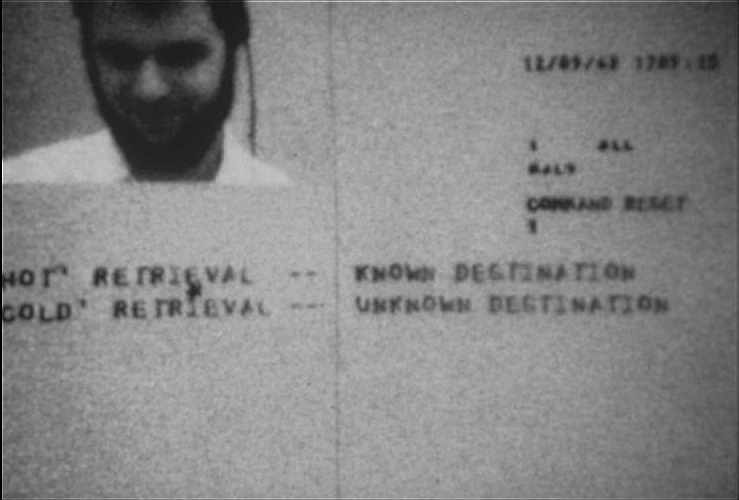
\includegraphics[width=0.5\textwidth]{images/first-videoconference}
\caption{Videoconferencing system in 1968. (source \cite{WIKI-HistoryOfVideoconferencing})}
\label{fig:FirstVideoconference1968}
\end{figure}

Nowadays, we are still used to the so-called \emph{desktop-to-desktop} communication paradigm: text messages exchanged through chat applications such as IRC, ICQ or Jabber, sound and image transmission using applications such as Skype or MS NetMeeting, which even allow for a limited multi-user videoconferences. There are, however, cases when these services simply do not suffice, when whole groups become participants in a session -- we call this the \emph{group-to-group} communication paradigm. The differences is immediately reflected to the increased hardware and software demands.
Each group usually utilizes multiple cameras and other visualization aids.
Especially the sound quality plays a dominant role in the conference rooms.
When groups are involved, the amount of intrusive effects such as echo rises significantly.

However, the usefulness of the technology is always limited by the simplicity, availability and affordability of the particular technology, regardless of the audience involved (groups of scientists, team members within a company, teachers and students).

Scientific workplaces and universities have always been connected to the fastest networks available to on market which led to the idea of utilizing the existing infrastructure for video-conferencing purposes. As an example could be the Masaryk University in Brno, where the video-conferencing node called AccessGrid Point was set up. Details can be found in the paper \cite{ArticleUVTMU-KomunikaceAGPoint}, where the authors E. Hladká and P. Holub refer to the possibility of extending the computational grids\footnote{Grid -- distributed system providing facilities to solve computationally complex problems using parallel algorithms such as physics of high energies, astrophysics and biology.} using devices enabling virtual meetings (video/conferences). Such principle has also been popular among founders of various grid-like projects, thus along with the grid infrastructure, also the AccessGrid network, composed of special videoconferencing rooms, facilitating distant high-quality collaboration, has been developed.

Within the text of this thesis, I would like to highlight alternative open-source solution as a counterpart to the expensive commercial applications available to date.
The main problem, however, is the simplicity of installation and management of such a heterogeneous and complex system. It is often easier for users to buy an expensive all-in-one solution than to adapt open-source applications.

\paragraph*{Main goals:}

\begin{enumerate}
%-------------------
\item To find a pure open-source-based solution providing video-conferencing capabilities for a group-to-group communication.
The system should run inside a UNIX-like environment, preferably on the Linux platform.

%-------------------
\item To implement session recording, editing and archiving.
\end{enumerate}

The central technology in this work is the AccessGrid project.
We are going to compare it to the other existing technologies, to discuss its advantages and drawbacks and to describe ideas and further improvements of the platform. As a proof-of-concept we built a real video-conference room which demonstrates the feasibility of our approach and hopefully brings the AccessGrid technology closer to ordinary users.